\chapter{Introduction}

\textbf{Author: Vor- und Nachname}

\vspace{2mm}

\lipsum[1-3]

\section{Section}
More text. \lipsum[1] See Figure~\ref{pic:example}.

\begin{figure}[h]
	\centering
	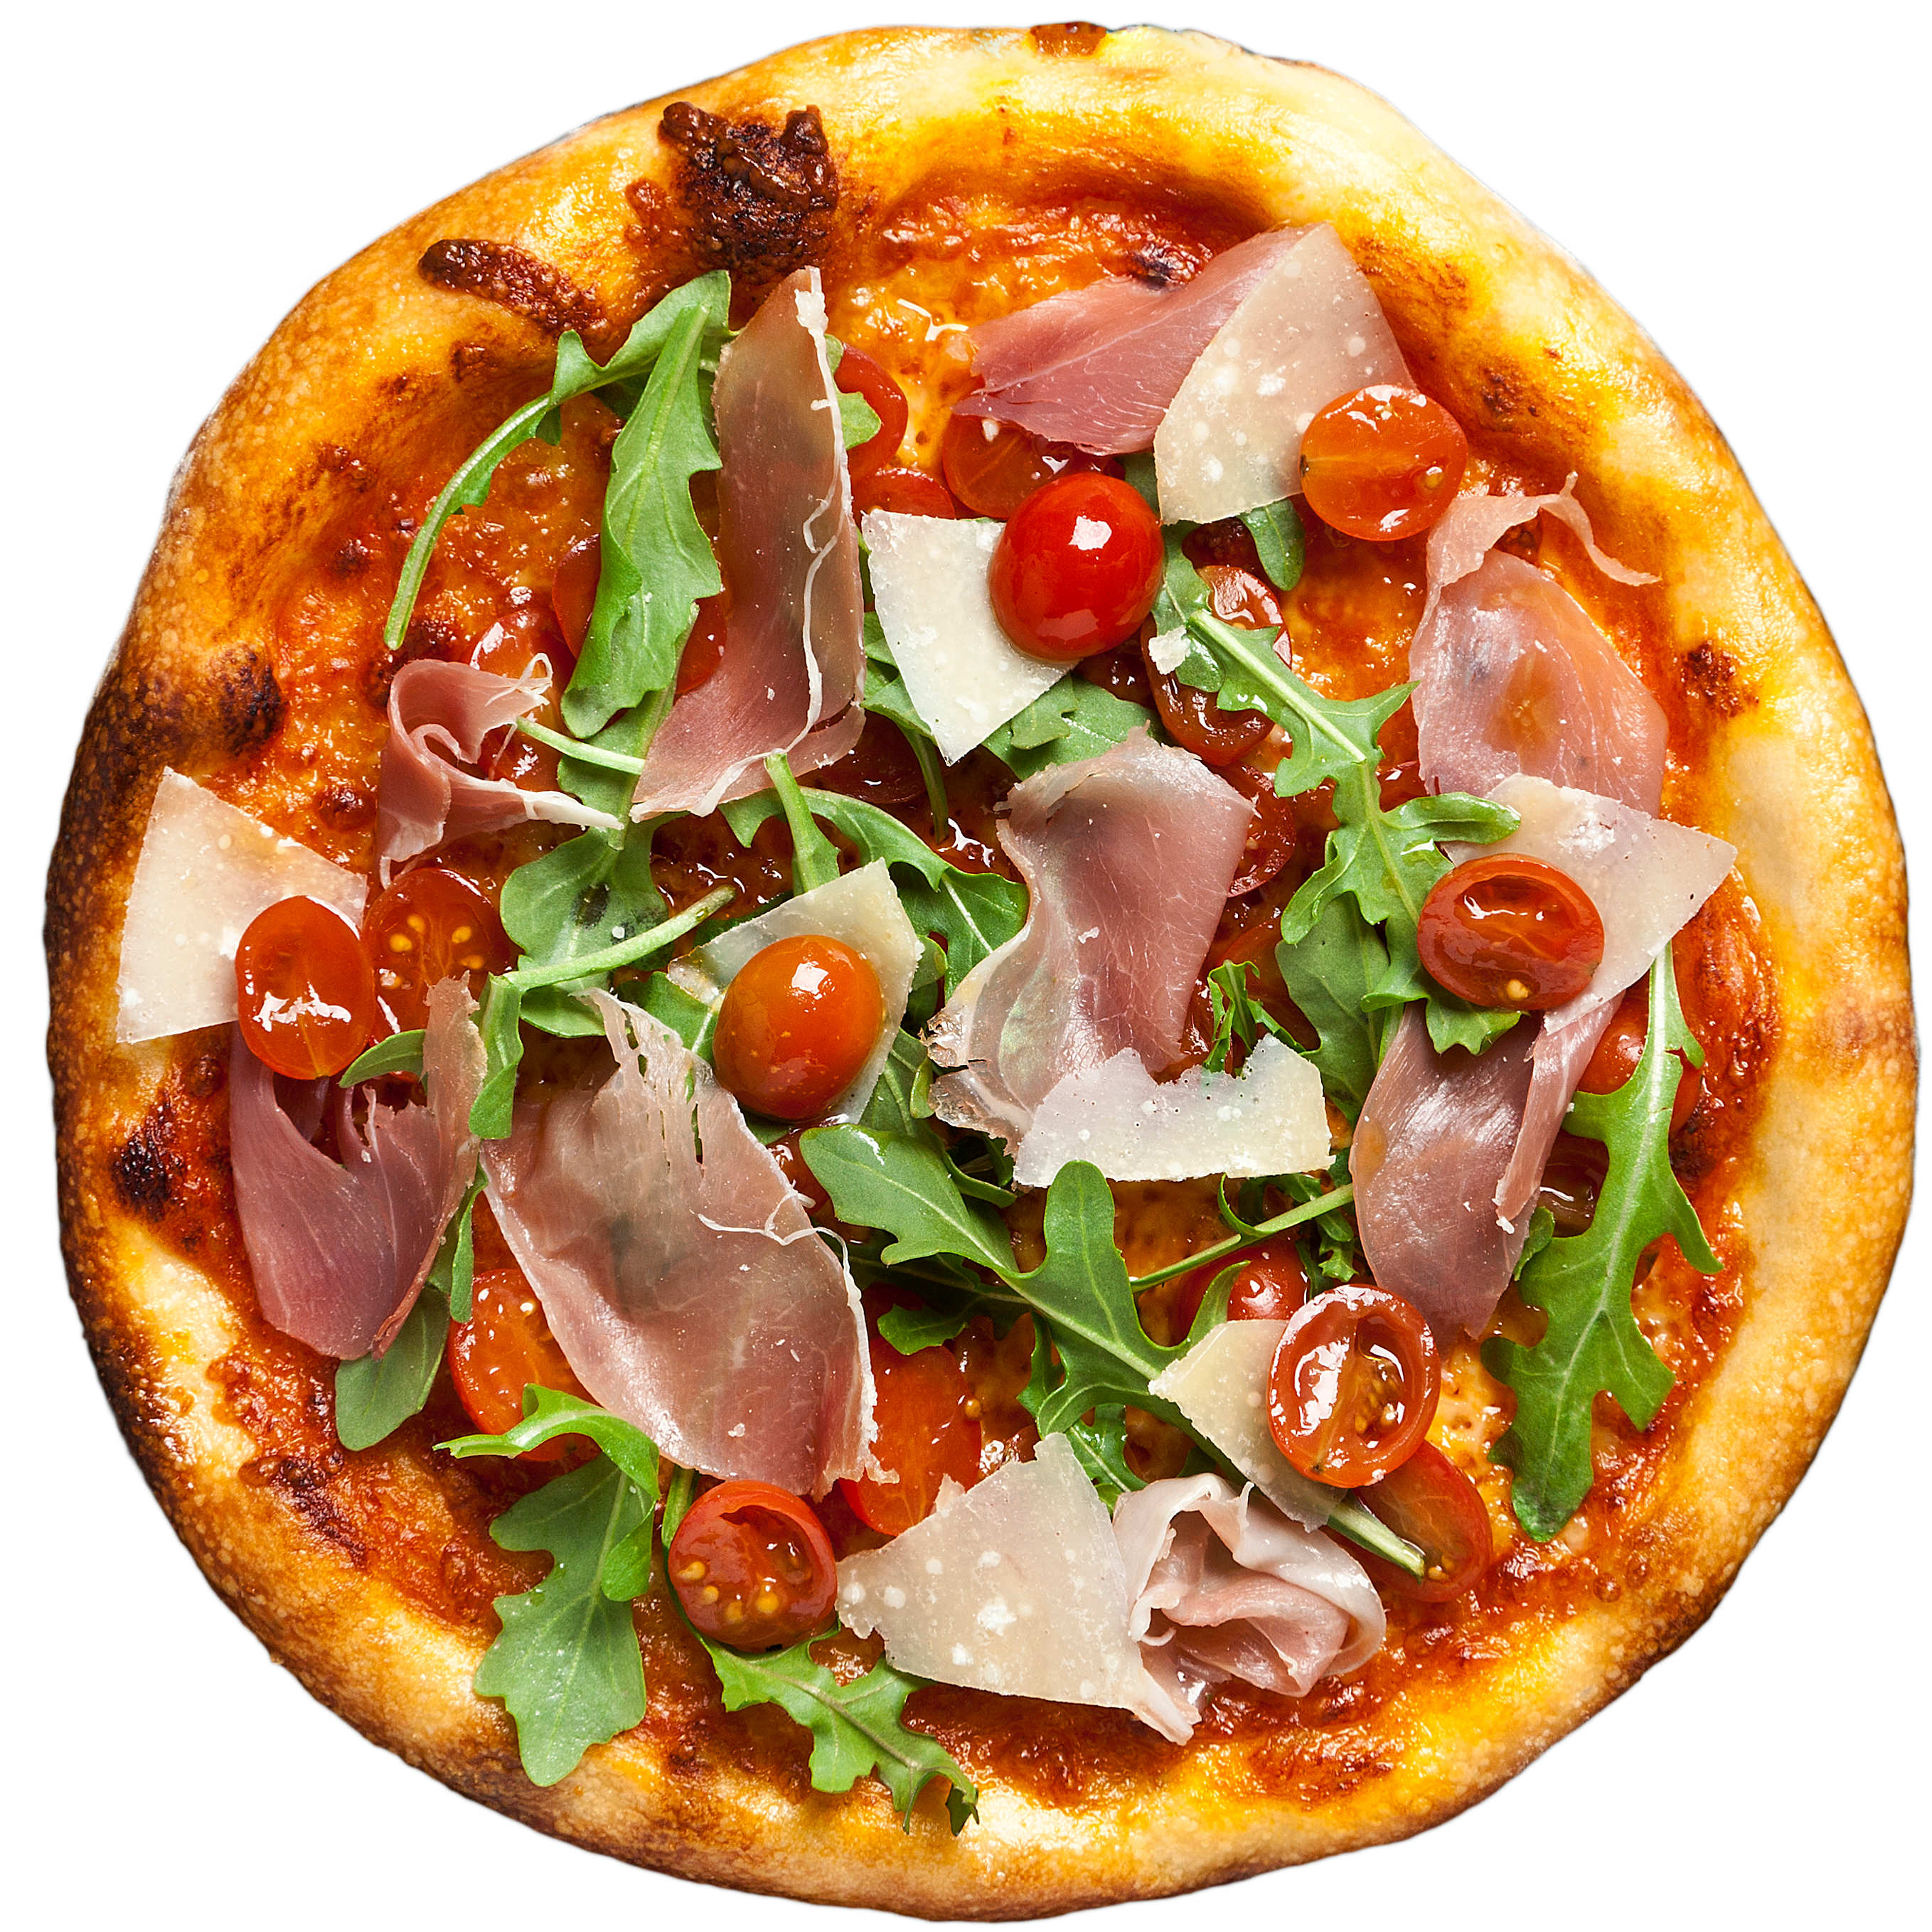
\includegraphics[width=2.5in]{img/example.png}
	\caption{Picture description.}
	\label{pic:example}
\end{figure}

\subsection{Subsection}
\lipsum[1]

\subsection{Subsection}
\lipsum[1] See Table~\ref{tab:example}.

\begin{center}
	\begin{tabular}{| l | l | l |}
		\hline
		\bfseries Header 1 & \bfseries Header 2 & \bfseries Header 2 \\
		\hline
		Text & text & text \\
		\hline
		Text & text & text  \\
		\hline
		Text & text & text  \\
		\hline
	\end{tabular}
	\label{tab:example}
\end{center}



\lipsum[1] Some references can be found at \footcite{robo4you} or at  \footcite{Hope_Learning_TensorFlow}. 


\filbreak
